\chapter{Prédictions de couverture et de débit}
\label{ch-pred}

Ce chapitre présente les livrables de prédiction du sujet sur le réseau initial (20 sites) : niveau de signal, couverture par émetteur et recouvrement, qualité C/(I+N), débits DL et UL. Chaque carte est l'export d'Atoll avec sa légende. Pour comparer chaque résultat aux objectifs \emph{par zone}, nous avons exporté les prédictions en raster (\SI{50}{\metre}) et écrit un script qui les croise avec les zones de l'Étape 1, en surface et en population. Le même script mesure ensuite chaque action d'optimisation.

\section{Niveau de signal}
\label{sec-signal}

La prédiction \enquote{Coverage by Signal Level (DL)} est calculée avec le seuil de \SI{-120}{\dBm}, l'effet de masque activé avec une probabilité de \SI{86}{\percent} au bord de la cellule (celle de la formule de Jakes, \cref{tab-jakes}) et une résolution de \SI{50}{\metre}. Deux versions ont été produites : indoor (objectif urbain) et outdoor (objectif rural).

\begin{figure}[H]
\centering
\begin{subfigure}[b]{0.58\textwidth}\centering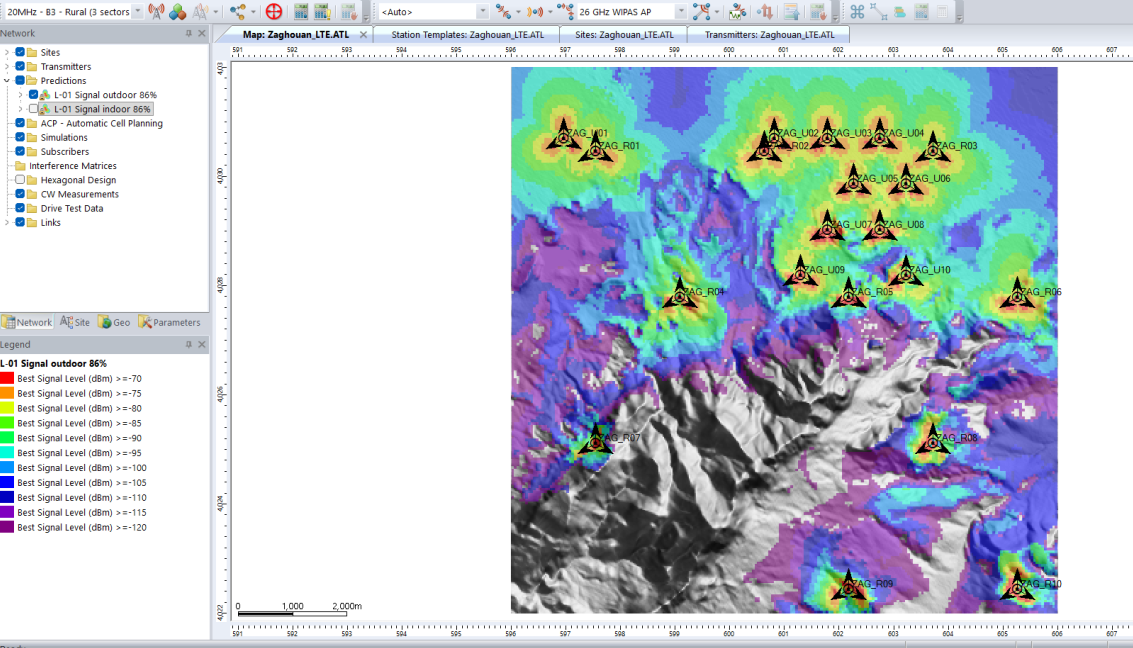
\includegraphics[width=\textwidth]{L-01_signal_outdoor_86_initial.png}\caption{Carte et légende Atoll, outdoor.}\end{subfigure}\hfill
\begin{subfigure}[b]{0.4\textwidth}\centering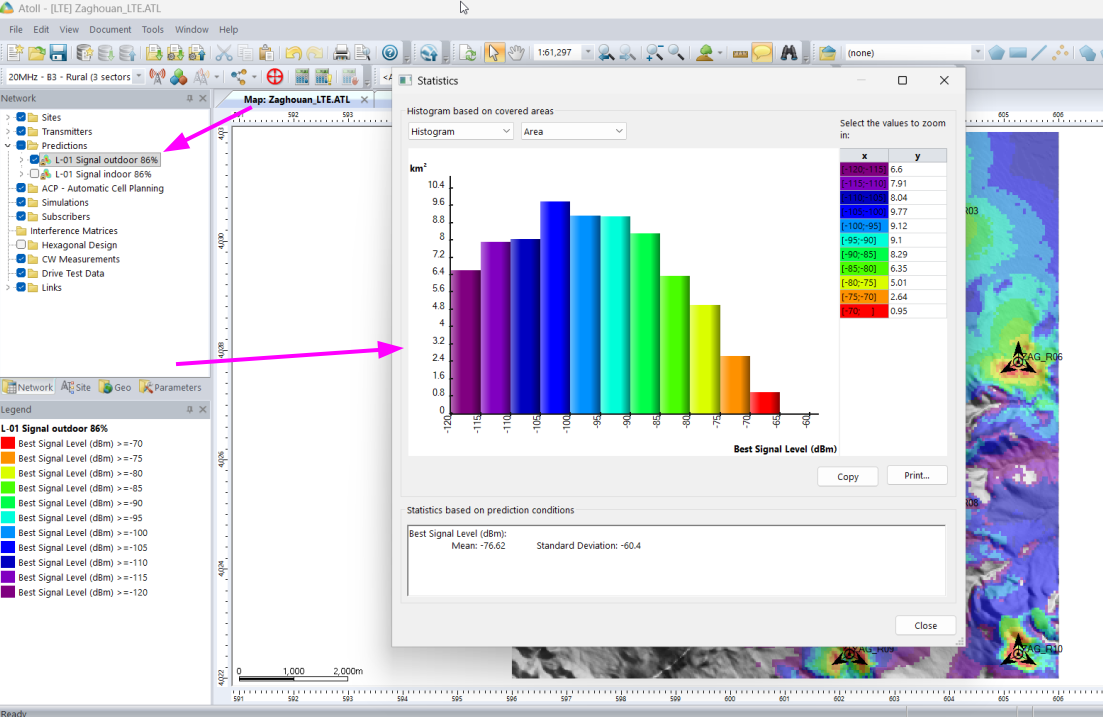
\includegraphics[width=\textwidth]{L-02_histogramme_outdoor_initial.png}\caption{Histogramme (surface par classe).}\end{subfigure}
\caption{Niveau de signal du réseau initial (outdoor).}
\label{fig-l1}
\end{figure}

L'histogramme donne \SI{59,1}{\kilo\metre\squared} au-dessus de \SI{-120}{\dBm} en indoor et \SI{73,8}{\kilo\metre\squared} en outdoor, sur les \SI{100}{\kilo\metre\squared} de la carte (massif compris). Par zone :

\begin{table}[H]
\centering
\caption{Couverture par niveau de signal du réseau initial.}
\label{tab-l1}
\small\setlength{\tabcolsep}{5pt}
\begin{tabular}{@{}lccccc@{}}
\toprule
\thead{Zone} & \thead{Mode} & \thead{Surface\\couverte} & \thead{Population\\couverte} & \thead{Objectif} & \thead{Verdict} \\
\midrule
Centre urbain & indoor & \SI{99,5}{\percent} & \SI{99,6}{\percent} & \SI{95}{\percent} & \ok \\
Rural & outdoor & \SI{83,4}{\percent} & \SI{95,4}{\percent} & \SI{95}{\percent} & \ko{} ($-11{,}6$ pts) \\
Massif & outdoor & \SI{7}{\percent} & -- & aucun & -- \\
\bottomrule
\end{tabular}
\end{table}

La ville est entièrement couverte en indoor. En campagne, il manque 11,6 points. Les trous se situent derrière le massif (\cref{fig-trous}) : le coin sud-ouest, où R07, placé sur le flanc, est masqué ; le pied est de la crête ; le sud-est, entre R08, R09 et R10. Ces zones sont peu peuplées : \SI{95,4}{\percent} des habitants ruraux sont couverts. L'objectif étant fixé en surface, il n'est pas atteint.

\begin{figure}[H]
\centering
\begin{subfigure}[b]{0.49\textwidth}\centering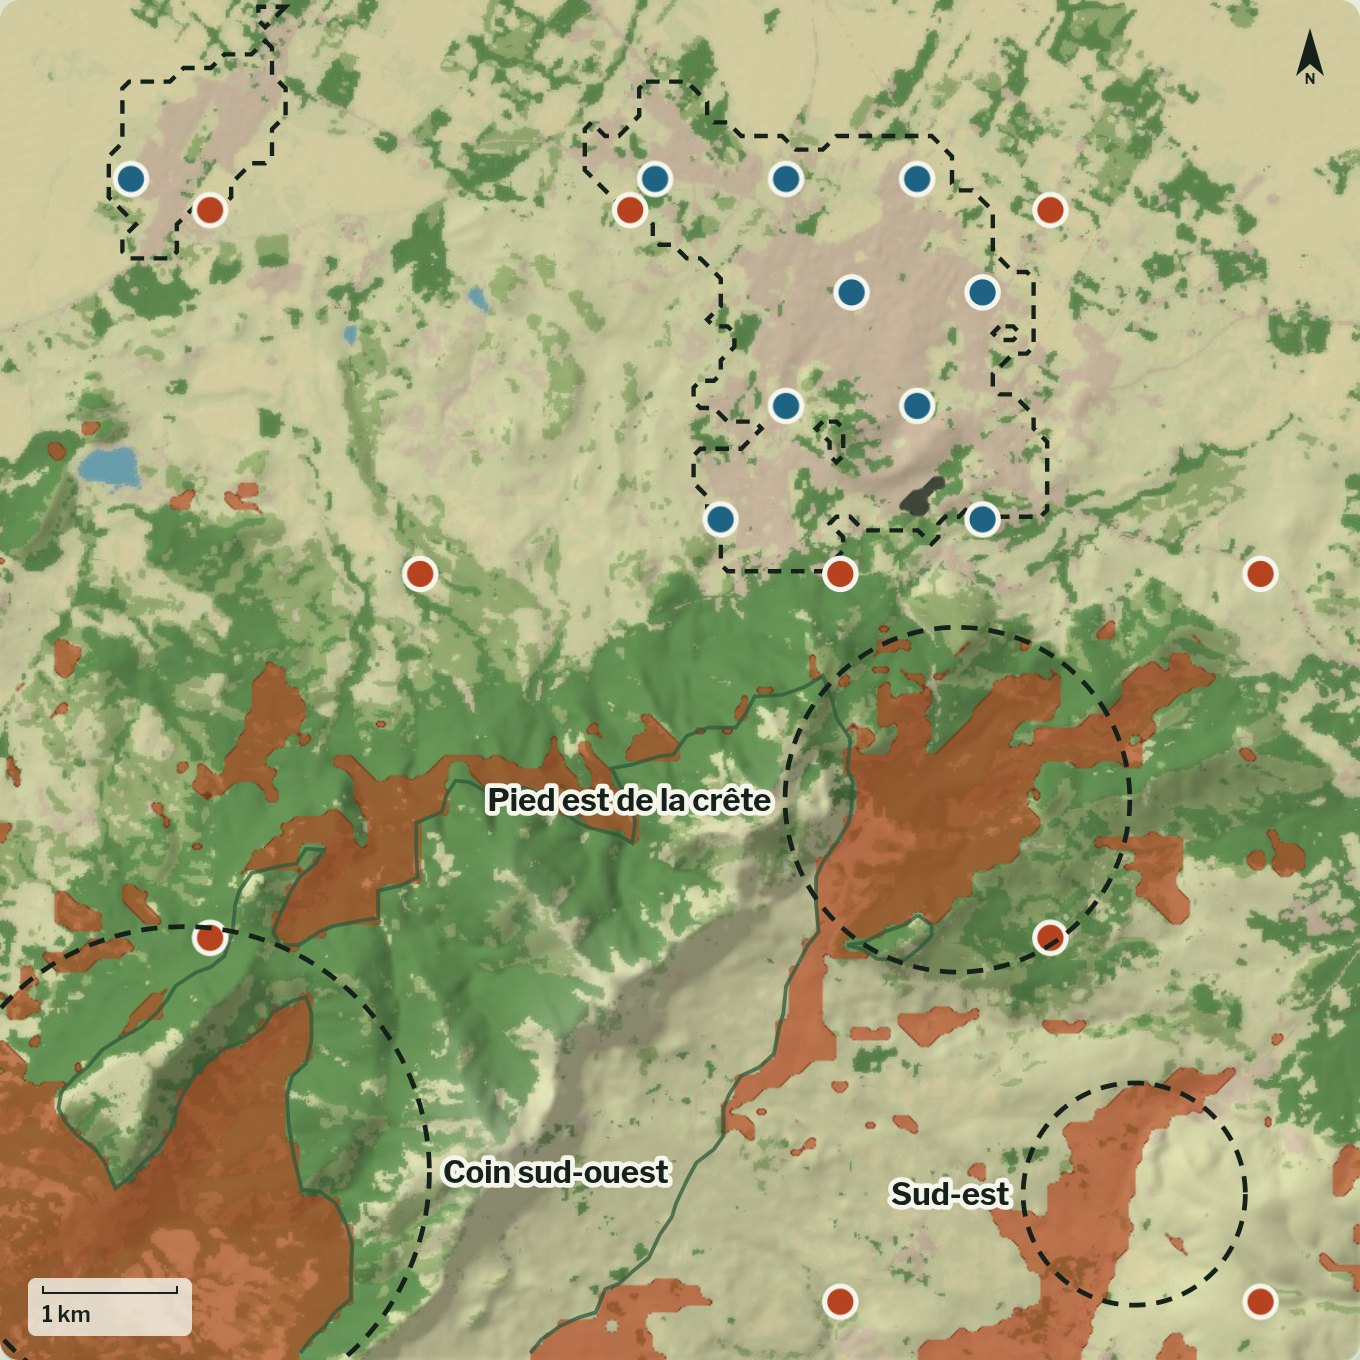
\includegraphics[width=\textwidth]{trous-initial.jpg}\caption{Trous de couverture rurale (en rouge).}\end{subfigure}\hfill
\begin{subfigure}[b]{0.49\textwidth}\centering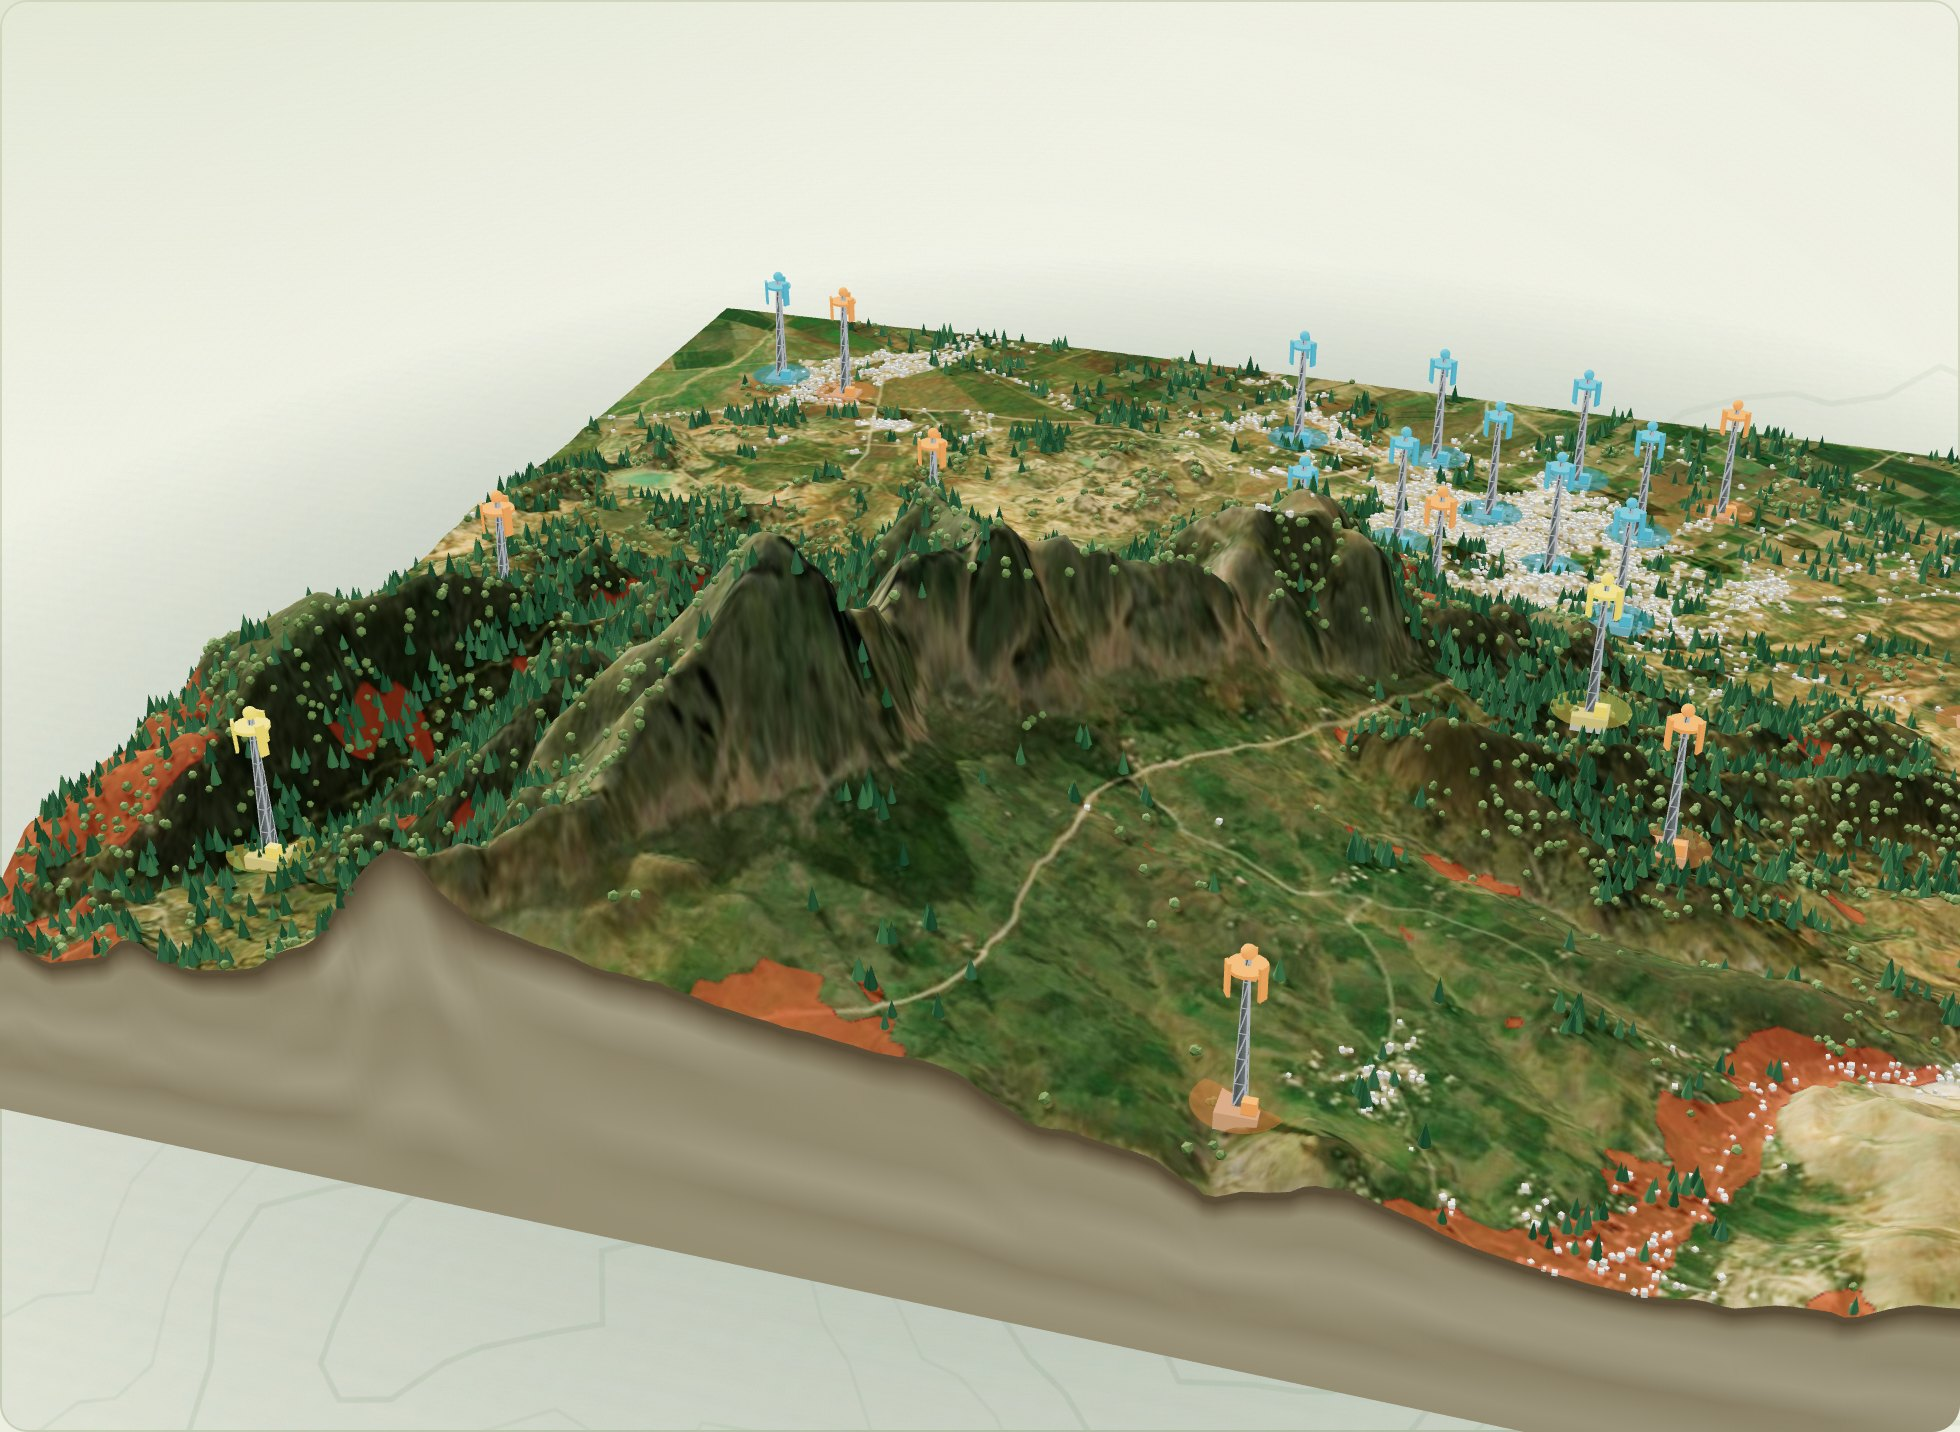
\includegraphics[width=\textwidth]{ombre-initial.jpg}\caption{Les mêmes trous drapés sur le relief réel.}\end{subfigure}
\caption{Trous de couverture rurale du réseau initial.}
\label{fig-trous}
\end{figure}

Les trous (en rouge) sont dans l'ombre de la crête. C'est la diffraction sur le relief, ignorée par la formule de Hata seule, qui les fait apparaître.

\section{Couverture par émetteur et recouvrement}
\label{sec-recouvrement}

La carte par émetteur (\cref{fig-l4}a) montre la zone servie par chaque cellule : les sites ruraux placés en hauteur (R04, R06) servent loin dans la plaine. La carte de recouvrement (\cref{fig-l4}b) compte, en chaque point, le nombre d'émetteurs reçus à moins de \SI{5}{\deci\bel} du meilleur.

\begin{figure}[H]
\centering
\begin{subfigure}[b]{0.49\textwidth}\centering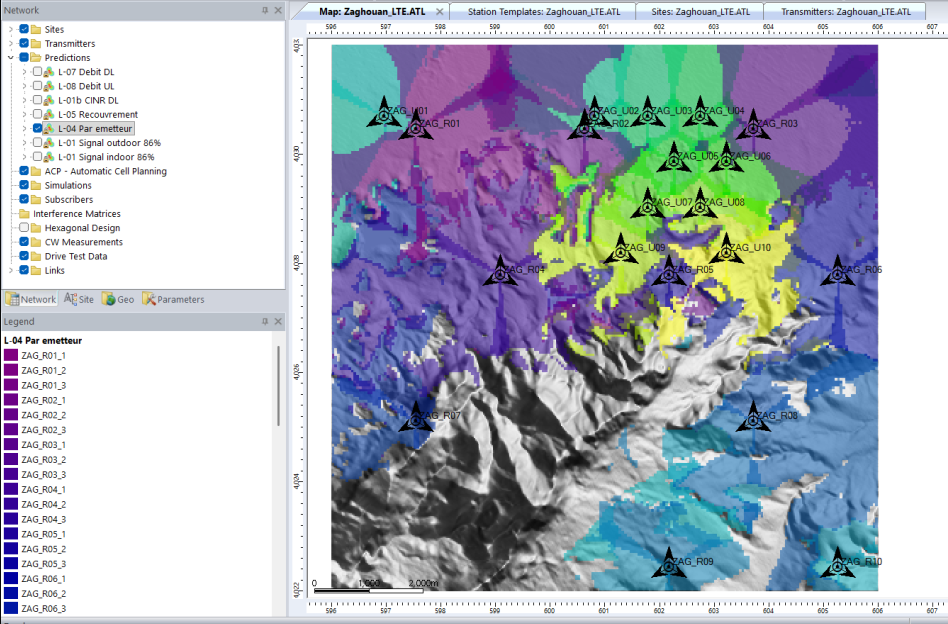
\includegraphics[width=\textwidth]{L-04_par_emetteur_initial.png}\caption{Couverture par émetteur.}\end{subfigure}\hfill
\begin{subfigure}[b]{0.49\textwidth}\centering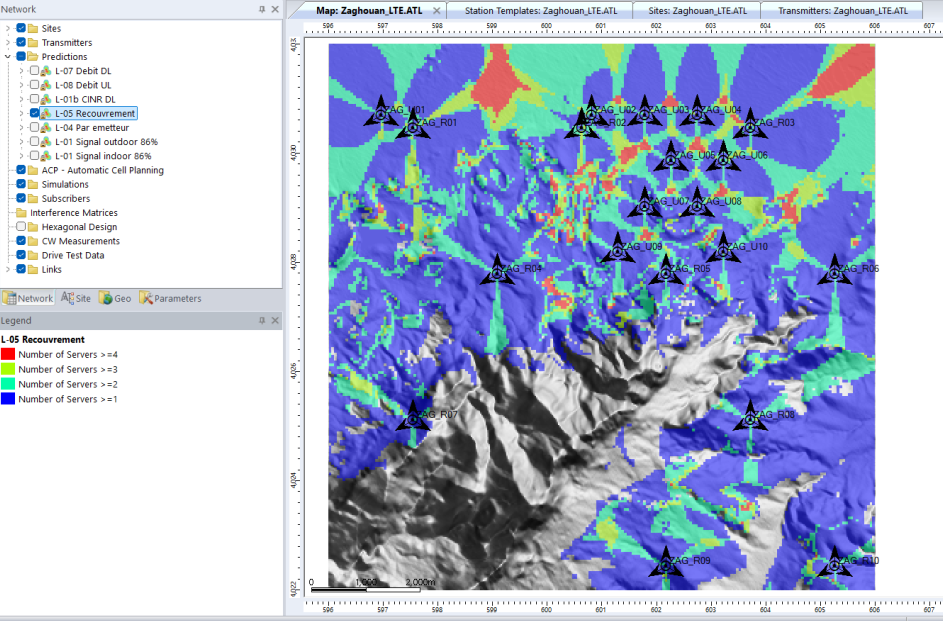
\includegraphics[width=\textwidth]{L-05_recouvrement_initial.png}\caption{Recouvrement (marge \SI{5}{\deci\bel}) et légende.}\end{subfigure}
\caption{Couverture par émetteur et recouvrement du réseau initial.}
\label{fig-l4}
\end{figure}

\begin{table}[H]
\centering
\caption{Histogramme de recouvrement du réseau initial.}
\label{tab-l5}
\begin{tabular}{@{}lccccc@{}}
\toprule
\thead{Nombre de serveurs} & \thead{1} & \thead{2} & \thead{3} & \thead{$\geq$ 4} & \thead{Total couvert} \\
\midrule
Surface (\si{\kilo\metre\squared}) & 48,85 & 17,83 & 4,70 & \textcolor{terre}{\textbf{2,39}} & 73,77 \\
\bottomrule
\end{tabular}
\end{table}

Avec une marge de \SI{5}{\deci\bel}, \SI{34}{\percent} de la surface couverte reçoit au moins deux serveurs à \SI{5}{\deci\bel} près (en moyenne 1,49 serveur). C'est utile pour le handover, mais en réutilisation~1 chaque serveur en trop est un interféreur. Les zones à quatre serveurs ou plus se situent dans la ville, entre U02 et U04, autour de U05 à U08 et près de R02.

\section{Qualité du signal : C/(I+N)}
\label{sec-cinr}

Un point couvert doit aussi recevoir un signal utile qui domine l'interférence. La prédiction C/(I+N) en DL (\cref{fig-cinr}) utilise la charge écrite dans la table des cellules, par défaut \SI{100}{\percent} pour les 60 cellules.

\begin{figure}[H]
\centering
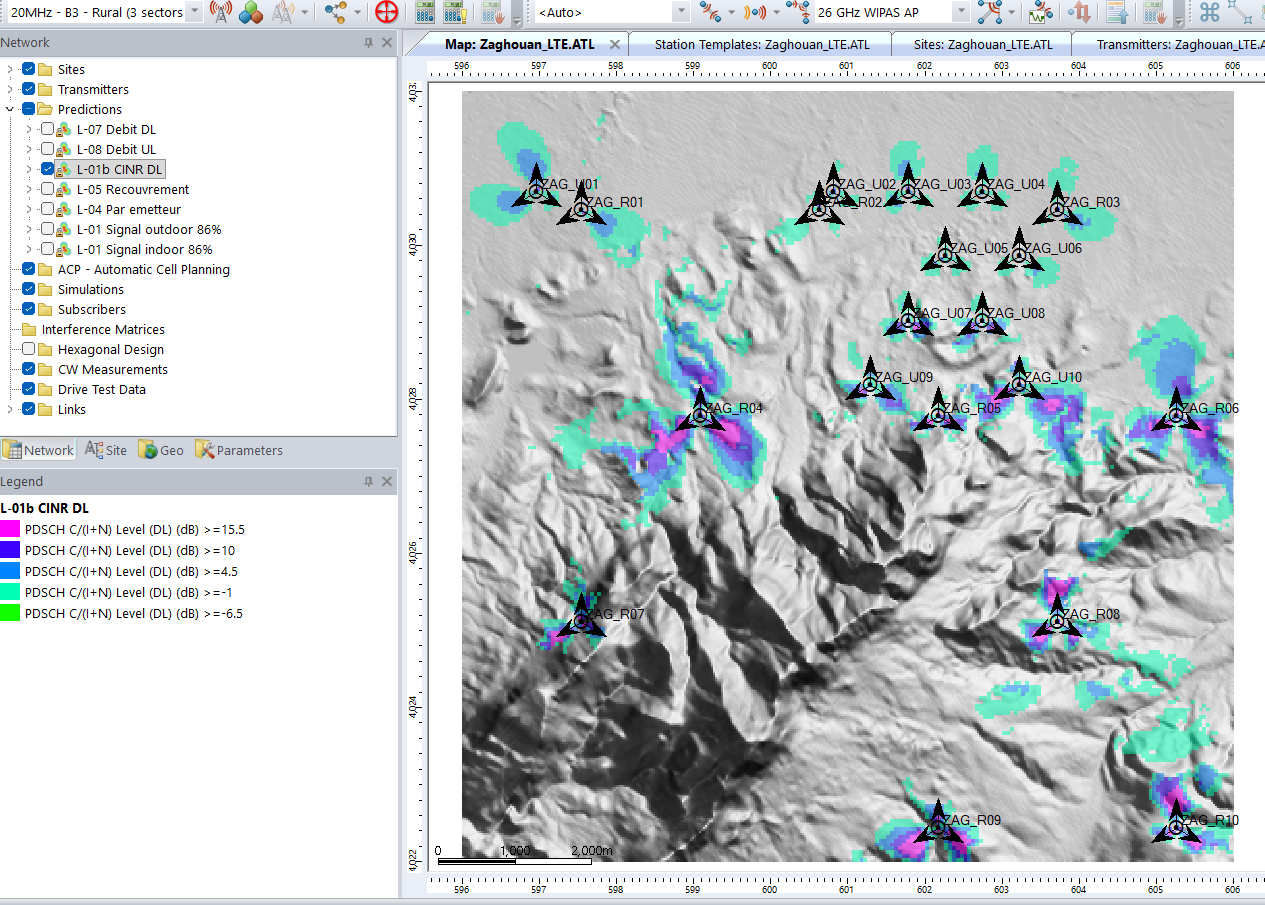
\includegraphics[width=0.7\textwidth]{L-01b_CINR_DL_initial.png}
\caption{C/(I+N) en DL du réseau initial (charge \SI{100}{\percent}).}
\label{fig-cinr}
\end{figure}

Sur la \cref{fig-cinr}, les zones blanches n'ont aucun bearer utilisable pour le service. Seuls \SI{13,1}{\kilo\metre\squared} atteignent \SI{-1}{\deci\bel}, le seuil du bearer~4 (moyenne \SI{4,9}{\deci\bel}). Le recouvrement l'explique : avec quatre serveurs reçus au même niveau, le signal utile fait face à trois interféreurs, soit $C/I = 1/3 \approx \SI{-5}{\deci\bel}$. C'est la limite de $K = 1$ annoncée par la formule du cours (formule~\eqref{eq-ci}, pire cas \SI{-12,6}{\deci\bel}), cette fois sur un relief réel. Trois causes ont été examinées séparément :
\begin{enumerate}
  \item \textbf{la géométrie des sites urbains} (recouvrement, tilt trop faible), traitée au \cref{ch-opt} ;
  \item \textbf{la charge de \SI{100}{\percent}} sur les 60 cellules, très pessimiste, remplacée plus loin par la charge simulée (\cref{sec-charge}) ;
  \item \textbf{la marge d'effet de masque} de \SI{86}{\percent}, qu'Atoll applique aussi au C/(I+N) : une prédiction sans cette marge agrandit nettement les zones de bonne qualité, mais les trous entre sites urbains restent. La cause principale est donc la géométrie.
\end{enumerate}
La même table des cellules fixe une montée du bruit en UL de \SI{0}{\deci\bel} : les prédictions UL ignorent donc l'interférence montante. Les cartes DL sont ainsi pessimistes et les cartes UL optimistes.

\section{Débits DL et UL}
\label{sec-debits}

Les prédictions de débit utilisent le service High Speed Internet (notre objectif de bord de cellule), un terminal MIMO, la mobilité piéton et les mêmes conditions d'effet de masque que le niveau de signal. Nous affichons le débit \emph{applicatif}, reçu par l'application après les erreurs de transmission et le facteur de 0,95 ; c'est lui qui se compare aux \SI{1024}{\kbps}. Les légendes commencent à l'objectif (\SI{1024}{\kbps} en DL, \SI{128}{\kbps} en UL), si bien qu'un point blanc dans la zone couverte est un point où l'objectif n'est pas atteint.

\begin{figure}[H]
\centering
\begin{subfigure}[b]{0.49\textwidth}\centering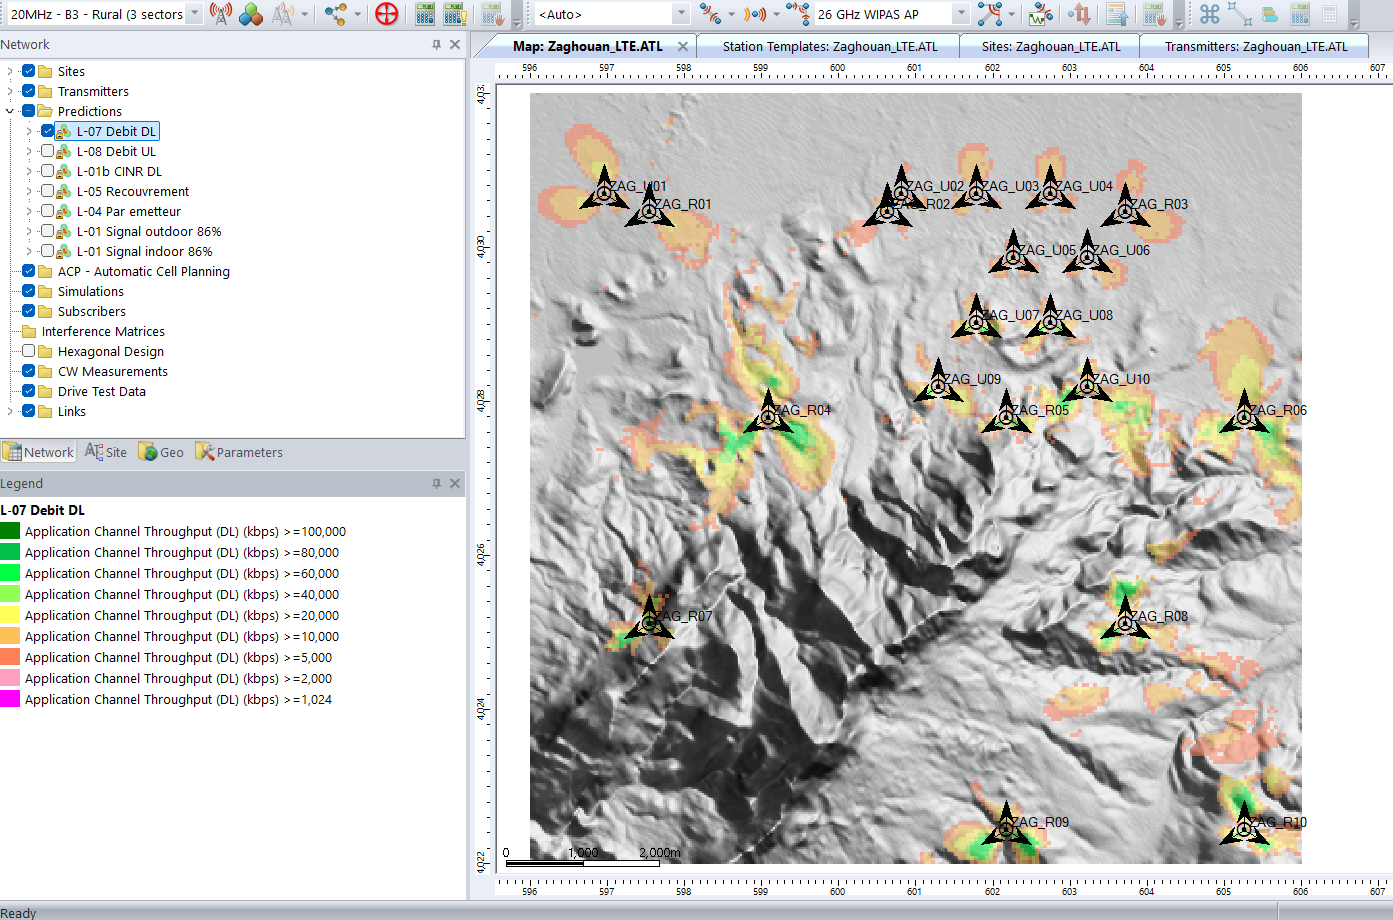
\includegraphics[width=\textwidth]{L-07_debit_DL_initial.png}\caption{Débit DL et légende.}\end{subfigure}\hfill
\begin{subfigure}[b]{0.49\textwidth}\centering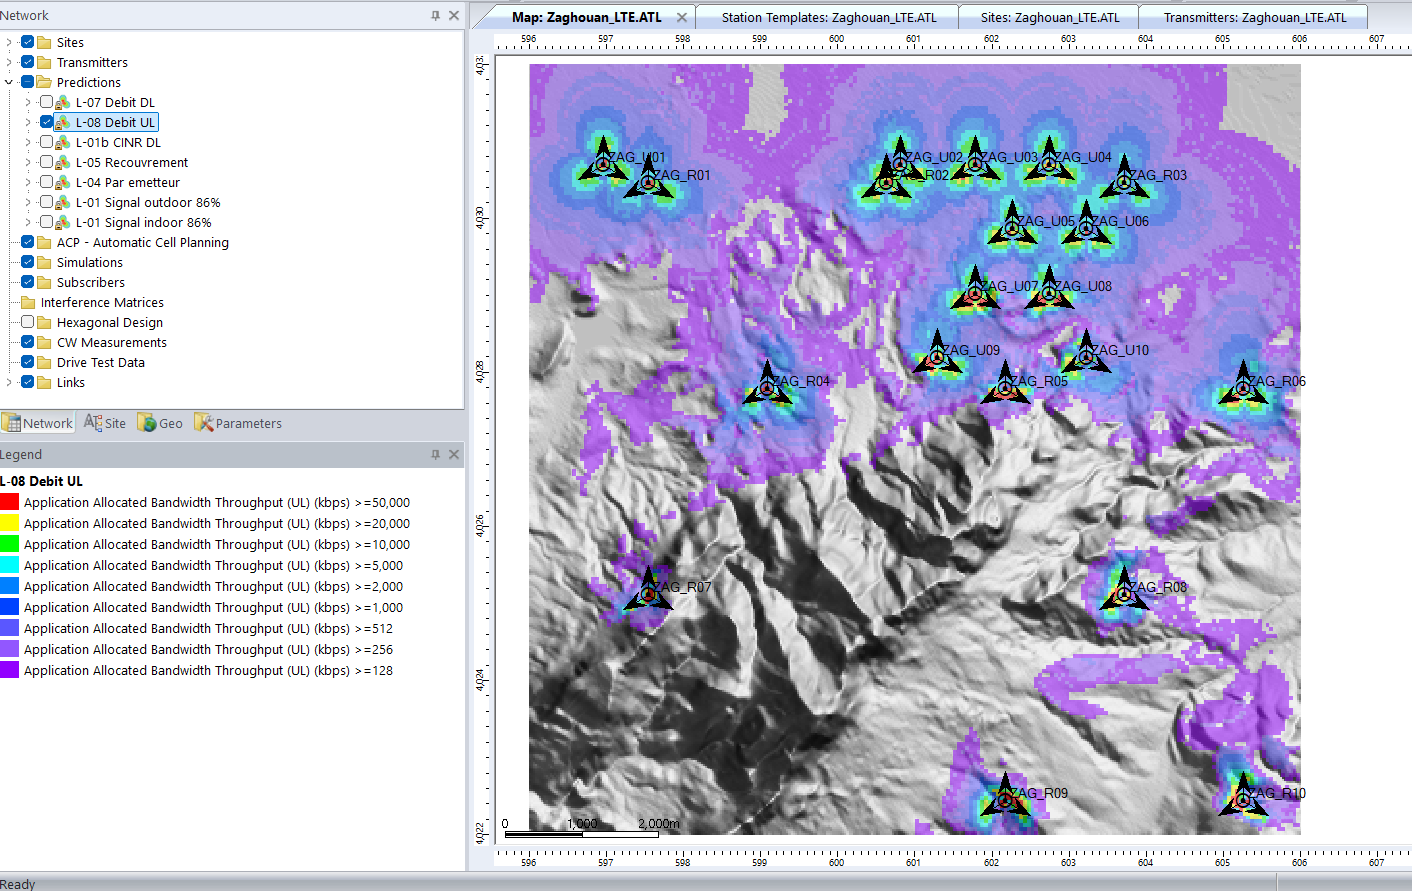
\includegraphics[width=\textwidth]{L-08_debit_UL_initial.png}\caption{Débit UL et légende.}\end{subfigure}
\caption{Débits applicatifs du réseau initial (charge \SI{100}{\percent}).}
\label{fig-debits}
\end{figure}

\begin{itemize}
  \item DL : \SI{13,1}{\kilo\metre\squared} reçoivent au moins \SI{1024}{\kbps}, exactement la surface où C/(I+N) $\geq \SI{-1}{\deci\bel}$. L'histogramme ne contient aucun pixel entre 1 et \SI{5}{\Mbps} : dès qu'un bearer existe, l'utilisateur dispose d'au moins \SI{5,8}{\Mbps} environ, ce que confirme notre calcul ($0{,}60$ bit/RE × 120 RE × 100 RB ≈ \SI{7,2}{\Mbps}, × 0,95, avant erreurs). En DL, c'est donc l'interférence qui décide de l'objectif.
  \item UL : \SI{48,6}{\kilo\metre\squared} reçoivent au moins \SI{128}{\kbps}. La limite est la puissance du terminal : en bord de cellule, il concentre ses \SI{23}{\dBm} sur quelques RB ; répartir sa puissance sur les 100 RB lui ferait perdre $10\log_{10}(100/2) \approx \SI{17}{\deci\bel}$ par RB.
\end{itemize}

\begin{table}[H]
\centering
\caption{Débits obtenus et débits cibles (réseau initial).}
\label{tab-l10}
\small\setlength{\tabcolsep}{5pt}
\begin{tabular}{@{}lcccc@{}}
\toprule
\thead{Sens} & \thead{Débit\\cible} & \thead{Surface atteignant\\la cible} & \thead{Débit moyen dans\\la zone servie} & \thead{Verdict} \\
\midrule
DL & \SI{1024}{\kbps} & \SI{13,1}{\kilo\metre\squared} (\SI{13}{\percent}) & \SI{18,7}{\Mbps} & \ko \\
UL & \SI{128}{\kbps} & \SI{48,6}{\kilo\metre\squared} (\SI{49}{\percent}) & -- & \ko \\
\bottomrule
\end{tabular}
\end{table}

\section{L'effet de la charge réelle}
\label{sec-charge}

La charge de \SI{100}{\percent} des prédictions est une valeur par défaut. Les simulations Monte-Carlo (\cref{ch-mc}) calculent la charge réelle de chaque cellule : à \num{1000} utilisateurs, \SIrange{4}{18}{\percent} pour les cellules urbaines et au plus \SI{30,7}{\percent} (la cellule R01\_1, qui sert le village du nord-ouest) ; la montée du bruit en UL reste sous \SI{0,5}{\deci\bel}. Atoll permet d'enregistrer ces charges dans la table des cellules ; les prédictions recalculées (sur le réseau après l'action 1 du \cref{ch-opt}) changent fortement :

\begin{figure}[H]
\centering
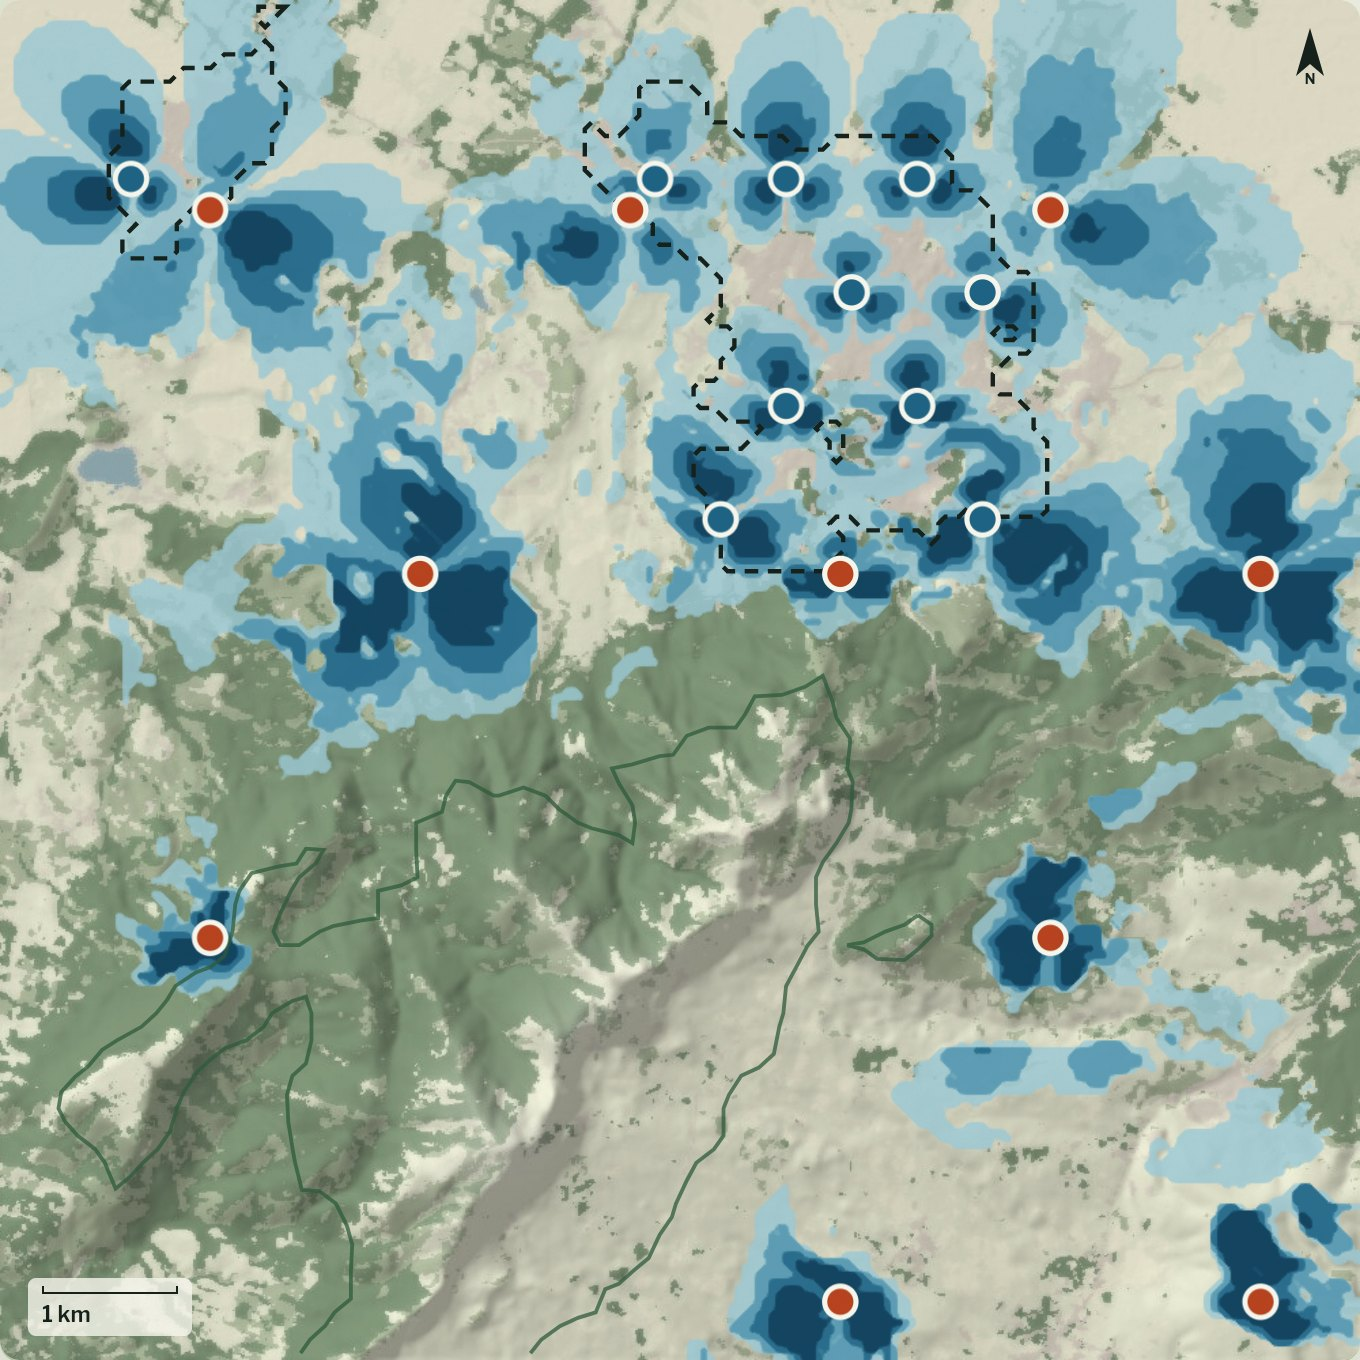
\includegraphics[width=0.56\textwidth]{cinr-mc1000.jpg}
\caption{C/(I+N) en DL avec les charges simulées.}
\label{fig-cinr-mc}
\end{figure}

Avec les charges de la simulation à \num{1000} utilisateurs (\cref{fig-cinr-mc}), la ville passe en grande partie au-dessus de \SI{-1}{\deci\bel}. Le \cref{tab-charge} compare les deux hypothèses sur le même réseau, avec les mêmes tilts.

\begin{table}[H]
\centering
\caption{Effet de la charge sur la qualité et les débits.}
\label{tab-charge}
\begin{tabular}{@{}lccc@{}}
\toprule
\thead{Indicateur} & \thead{Charge \SI{100}{\percent}} & \thead{Charge simulée} & \thead{Évolution} \\
\midrule
Surface C/(I+N) $\geq \SI{-1}{\deci\bel}$ & \SI{14,6}{\kilo\metre\squared} & \SI{36,1}{\kilo\metre\squared} & × 2,5 \\
C/(I+N) moyen & \SI{5,1}{\deci\bel} & \SI{6,6}{\deci\bel} & +\SI{1,5}{\deci\bel} \\
Débit DL moyen (zone servie) & \SI{18,7}{\Mbps} & \SI{34,0}{\Mbps} & \\
\bottomrule
\end{tabular}
\end{table}

En réutilisation~1, l'interférence reçue est proportionnelle à la charge des cellules voisines : passer de \SI{100}{\percent} à moins de \SI{20}{\percent} multiplie par 2,5 la surface utilisable en DL. Par zone, avec la charge simulée, la ville atteint \SI{99,5}{\percent} en UL ($\geq \SI{128}{\kbps}$) mais seulement \SI{78,9}{\percent} en DL ($\geq \SI{1}{\Mbps}$) ; la campagne atteint \SI{55,8}{\percent} en UL et \SI{38,0}{\percent} en DL.

\begin{retenir}
Il reste deux problèmes distincts : l'interférence entre sites urbains, qui limite le DL en ville, et la couverture derrière le massif, sur laquelle la charge n'a aucun effet.
\end{retenir}
